%&"../ml"
\begin{document}
    \title{第三次作业}
    \maketitle
    \section{SVM 与神经网络}

    \subsection{数据集信息}

    对两个数据集进行测试,其规模如表 \ref{tab:dataset} 所示。其中 madelon 数据集特征维度多,训练集大小大于测试集大小;ijcnn1 数据集特征维度相对较少,但是数据集规模大,测试集大小大于训练集大小。

    \begin{table}[ht]
        \centering
        \caption{数据集信息}\label{tab:dataset}
        \begin{tabular}{crrr}
            \toprule
            数据集   & 训练集大小 & 测试集大小 & 特征维度 \\
            \midrule
            madelon & 2000 & 600 & 500 \\
            ijcnn1 & 49990 & 91701 & 22 \\
            \bottomrule
        \end{tabular}
    \end{table}

    \subsection{与 MLP 的比较}

    数据读取实现于 \filelink{src/utils.py},特征将会被首先归一化再进行训练。SVM 实现于 \filelink{src/svm.py},具体参数为
    
    \codeseg[language=python]{src/svm.py}{12}{12}
    
    MLP 实现于 \filelink{src/mlp.py},具体参数为
    
    \codeseg[language=python]{src/mlp.py}{12}{12}
    
    表 \ref{tab:mlp} 展示了默认参数下 SVM 与 MLP 的效果。从准确率来看,SVM 的准确率在 madelon 多特征维度数据集上略高于 MLP,在 ijcnn1 向本较多的数据集上低于 MLP。训练时间上 SVM 收敛需要的时间也偏长,当然从后文可以看到这个时间可以通过调节参数的方式缩短。
    
    \begin{table}[ht]
        \centering
        \caption{SVM 与 MLP}\label{tab:mlp}
        \begin{tabular}{ccccc}
            \toprule
            \multirow{2}{*}{数据集} & \multicolumn{2}{c}{准确率} & \multicolumn{2}{c}{训练时间 (s)} \\
            \cmidrule(r){2-3}\cmidrule(l){4-5}
            & SVM & MLP & SVM & MLP \\
            \midrule
            madelon & \textbf{0.585} & 0.583 & 71 & 19 \\
            ijcnn1 & 0.919 & \textbf{0.961} & 130 & 91 \\
            \bottomrule
        \end{tabular}
    \end{table}

    \subsection{不同的核函数}

    表 \ref{tab:kernel} 展示了使用不同核函数的结果。其中在多维度的 madelon 上 linear 核的表现最好,但是训练时间较长,使用其它核会略微降低一点准确率,但是时间可以减少一个数量级。在少一些维度的 ijcnn1 上,rbf 的准确率最高,可以超过表 \ref{tab:mlp} 的 MLP,此时的 poly 核是更好的性价比选择。

    \begin{table}[ht]
        \centering
        \caption{SVM 不同核函数,$C=1$}\label{tab:kernel}
        \begin{tabular}{ccccccccc}
            \toprule
            \multirow{2}{*}{数据集} & \multicolumn{4}{c}{准确率} & \multicolumn{4}{c}{训练时间 (s)} \\
            \cmidrule(r){2-5}\cmidrule(l){6-9}
            & linear & poly & rbf & sigmoid & linear & poly & rbf & sigmoid \\
            \midrule
            madelon & \textbf{0.585} & 0.578 & 0.582 & 0.583 & 76 & 5  & 7 & 5 \\
            ijcnn1 & 0.919 & 0.948 & \textbf{0.968} & 0.867 & 150 & 70 & 141 & 127 \\
            \bottomrule
        \end{tabular}
    \end{table}

    \subsection{不同的 $C$}

    表 \ref{tab:c} 展示了不同的 $C$ 对 linear SVM 的影响,$C$ 将控制对软间隔的容忍度。可见其对准确率不会有特别大的影响,但是在训练时间上会有差异。同等准确率的情况下,对 madelon 而言,$C=0.1$ 最好;对 ijcnn1 而言,$C=0.1$ 最好。

    \begin{table}[ht]
        \centering
        \caption{不同的 $C$,linear}\label{tab:c}
        \begin{tabular}{ccccccccc}
            \toprule
            \multirow{2}{*}{数据集} & \multicolumn{4}{c}{准确率} & \multicolumn{4}{c}{训练时间 (s)} \\
            \cmidrule(r){2-5}\cmidrule(l){6-9}
            & 0.01 & 0.1 & 0.5 & 1 & 0.01 & 0.1 & 0.5 & 1 \\
            \midrule
            madelon & 0.568 & \textbf{0.585} & 0.57 & \textbf{0.585} & 5 & 9  & 29 & 71 \\
            ijcnn1 & 0.918 & \textbf{0.919} & \textbf{0.919} & \textbf{0.919} & 87 & 104 & 121 & 188 \\
            \bottomrule
        \end{tabular}
    \end{table}

    \section{因果发现算法}

    \subsection{数据集}

    导致肺癌的因素很多,本题将采用 LUCAS (LUng CAncer Simple set) 数据集\cite{lucas},来计算这个数据集 12 个因素(如表 \ref{tab:factors})之间的因果关系图。这 12 个因素都被编码为 0/1 值,共 2000 行。

    \begin{table}[ht]
        \centering
        \caption{因素}\label{tab:factors}
        \begin{tabular}{cll}
            \toprule
            序号 & 英语名 & 中文名 \\
            \midrule
            0  & Lung Cancer & 肺癌\\
            1  & Smoking &  吸烟 \\
            2  & Yellow\_Fingers & 黄手指  \\
            3  & Anxiety & 焦虑 \\
            4  & Peer\_Pressure & 同辈压力 \\
            5  & Genetics & 基因 \\
            6  & Attention\_Disorder & 注意力紊乱 \\
            7  & Born\_an\_Even\_Day &  在偶数日出生 \\
            8  & Car\_Accident & 车祸 \\
            9  & Fatigue & 疲劳 \\
            10 & Allergy & 过敏 \\
            11 & Coughing & 咳嗽 \\
            \bottomrule
        \end{tabular}
    \end{table}

    \subsection{算法}

    这里采用 LiNGAM(Linear Non-Gaussian Acyclic Model) 算法\cite{lingam},该算法假设变量满足
    \begin{equation}\label{eq:sem}
        x_i = \sum_{j:\text{parents of} i} b_{ij}x_j + e_i    
    \end{equation}
    并有如下假设:
    \begin{enumerate}
        \item 因果图为有向无环图(DAG)
        \item 外部影响 $e_i$ 都是非零方差的、并且独立非高斯
        \item 假设不存在 latent confounders
    \end{enumerate}
    假设 1 与 3 在图 \ref{fig:answer} 中也可以看到都是正确的。假设 2 根据数据描述也被认为是正确的。

    \paragraph{ICA}

    对于输入的数据矩阵 $\mathbf{X}$,每一列为一个样本向量 $\mathbf{x}$,归一化消去偏置后,将公式 \eqref{eq:sem} 进行转换,使用矩阵形式得到
    \begin{equation}
        \mathbf{x} = \mathbf{B}\mathbf{x} + \mathbf{e}
    \end{equation}
    需要对 $\mathbf{x}$ 进行求解
    \begin{equation}
        \mathbf{x} = (\mathbf{I} - \mathbf{B})^{-1}\mathbf{e} = \mathbf{W}^{-1}\mathbf{e}
    \end{equation}
    这将利用 ICA (Fast-ICA) 求解唯一的 $\mathbf{W}$,然后对排序得到对角线不为零的矩阵 $\tilde{\mathbf{W}}$,归一化对角元素得到 $\tilde{\mathbf{W}}^\prime$。从而估计权重矩阵 $\hat{\mathbf{B}} = \mathbf{I}-\hat{\mathbf{W}}^\prime$。

    \paragraph{排序}

    为了一一对应 $x_i$ 与 $e_i$ 对应,我们需要对 $\hat{\mathbf{B}}$ 进行排序,可以表示为 $\tilde{\mathbf{B}} = \mathbf{P}\hat{\mathbf{B}}\mathbf{P}^T$,$\tilde{\mathbf{B}}$ 接近于一个严格的下三角矩阵。从而得到一个有向无环图。

    \paragraph{剪枝}

    删去不重要的边以得到最终结果。

    \subsection{结果}

    参考这篇博客\cite{draw},在 Tetrad \cite{tetrad} 建立如图 \ref{fig:flow} 所示的流程图。

    \begin{figure}[ht]
        \centering
        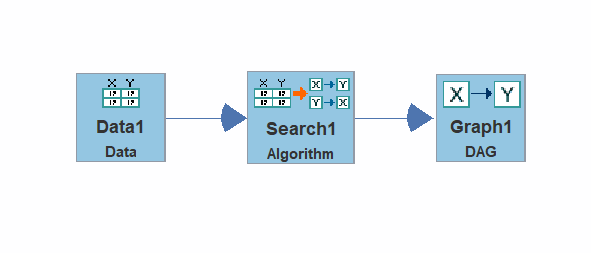
\includegraphics[width=7cm]{flow.png}
        \caption{流程图}\label{fig:flow}
    \end{figure}
    
    最后推断结果如图 \ref{fig:result} 所示。这个结果可以与生成数据的标准答案图 \ref{fig:answer} 做对比。可以发现有些联系方向依然有一些问题,比如
    \fbox{Car Accident}$\rightarrow$\fbox{Genetics} 和 \fbox{Car Accident}$\rightarrow$\fbox{Attention Disorder}
    关系明显可以用已有知识判定为错误。在 \fbox{Lung Cancer}$\rightarrow$\fbox{Smoking},\fbox{Lung Cancer}$\rightarrow$\fbox{Genetics},\fbox{Lung Cancer}$\rightarrow$\fbox{Fatigue},\fbox{Smoking}$\rightarrow$\fbox{Anxiety},\fbox{Smoking}$\rightarrow$\fbox{Peer Pressure} 等为相反方向,\fbox{Genetics}$\rightarrow$\fbox{Smoking},\fbox{Fatigue}$\rightarrow$\fbox{Allergy},\fbox{Fatigue}$\rightarrow$\fbox{Attention Disorder} 为新增边。

    大部分的框架仍然是很明晰的,而部分错误结果与 ICA-LiNGAM 算法的缺陷有一定的关系,使用 FastICA 算法可能收敛到局部最优解,变量排序可能因尺度发生变化。此算法的进阶版本为 Direct LiNGAM,可以接受先验知识也可以得到更加可靠的结果,但也会导致更高的算法复杂度。由于 Tetrad 并没有实现 Direct LiNGAM,此处无法引入先验知识,只采用了 ICA-LiNGAM 求解。

    \begin{figure}[ht]
        \centering
        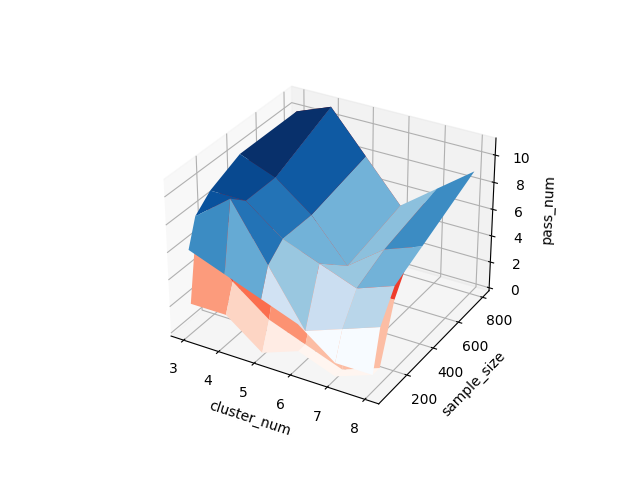
\includegraphics[width=0.7\textwidth]{result.png}
        \caption{因果推断结果}\label{fig:result}
    \end{figure}

   
    \begin{figure}[ht]
        \centering
        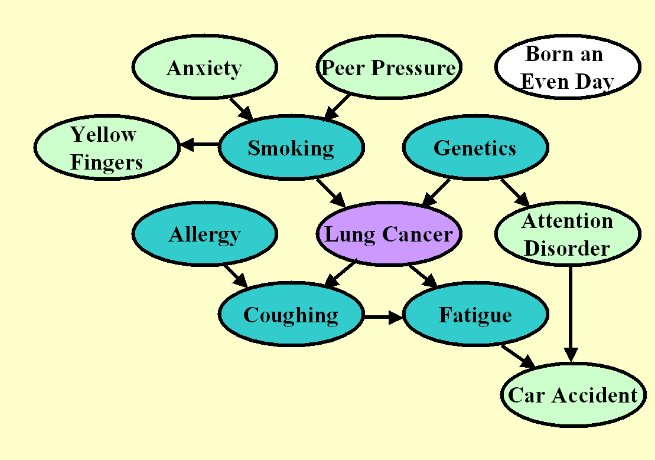
\includegraphics[width=0.7\textwidth]{answer.png}
        \caption{生成数据的依赖图}\label{fig:answer}
    \end{figure}

    \bibliography{ref}

\end{document}